\chapter{Investor and Executive Doug Williams: Focus, Scale, and Character}

The source for this chapter is the School of Hard Knocks interview with Doug Williams, curated for these notes by LazyingArt LLC. Williams speaks as a former chief operating officer of HMS Holdings, a healthcare company he says was sold for about \(\$3.5\) billion, and as a current investor and board member. The mathematics here is therefore commercial mathematics: scale, thresholds, ratios, valuation multiples, operating sequences, and the disciplined separation between anecdote, claim, and mechanism.

\section{Investment Filters Before Investment Stories}

The interview opens with a credential, but it does not stay there. Williams is introduced through HMS Holdings and the \(\$3.5\) billion sale, then the first substantive question asks what he looks for in a startup. The order matters. The large exit gives standing; the investment filter gives method.

He describes an investment company with roughly
\begin{equation}
C_{\mathrm{fund}} \approx \$50\,\mathrm{M}
\end{equation}
available to invest. The fund is venture-oriented and early-stage. Typical checks are approximately
\begin{equation}
\$0.5\,\mathrm{M} \lesssim I_{\mathrm{check}} \lesssim \$3\,\mathrm{M},
\end{equation}
and the target companies are often still below roughly
\begin{equation}
R_{\mathrm{startup}} \lesssim \$2\,\mathrm{M}
\end{equation}
in revenue.

Those numbers do not replace judgment. They locate the kind of uncertainty Williams is talking about. At that stage, he looks for interesting ideas, thoughtful management teams, and large target markets. Then the investor's work becomes operational: focus the company, help it hire talent, and keep the team aimed at the few things that matter.

\begin{table}
\centering
\begin{tabular}{p{.38\linewidth}p{.5\linewidth}}
Object & Transcript-grounded value or criterion \\
Fund capacity & about \(\$50\,\mathrm{M}\) \\
Typical check & about \(\$0.5\,\mathrm{M}\) to \(\$3\,\mathrm{M}\) \\
Company revenue & probably below \(\$2\,\mathrm{M}\) \\
Investment stage & early venture rounds \\
Qualitative filter & idea, team, and large target market \\
Investor work & focus, talent, organization, discipline \\
\end{tabular}
\end{table}

So the first move is from money to attention. Capital is necessary, but at this stage capital is not enough. A young company can have more possible tasks than it has people. The investor who only writes a check has not yet solved the operating problem.

\section{From Smart Founder to Sellable Message}

Williams next gives a coaching example. A founder may be smart, know the market, and understand the product set. Still, the message can fail. It may not be focused enough; it may not tell the buyer why the issue matters now.

This is where Williams introduces one of the interview's sharpest claims: sell through fear, not foresight. We should read this carefully. He is not giving a license to scare customers indiscriminately. His narrower claim is that executives are often more motivated by preventing failure than by imagining upside. If the seller can connect the product to a failure the buyer already has reason to avoid, the message becomes concrete.

\subsection{Question \& Answer}

\paragraph{Question.} Why would a very large customer listen to a very small company?

\paragraph{Answer.} Because the small company can be connected to a problem the customer cannot afford to ignore, and because trust can be transferred from a credible person to an otherwise unfamiliar firm. Williams makes the asymmetry explicit with a small company selling into a much larger one:
\begin{equation}
S_{\mathrm{seller}} \approx \$2\,\mathrm{M},
\qquad
S_{\mathrm{buyer}} \approx \$50\,\mathrm{B}.
\end{equation}
As a scale comparison, this is about
\begin{equation}
\frac{S_{\mathrm{buyer}}}{S_{\mathrm{seller}}}
\approx
\frac{50\,\mathrm{B}}{2\,\mathrm{M}}
=
25{,}000.
\end{equation}
The ratio is a reconstruction, not a number Williams computes aloud. It is useful because it makes the credibility gap visible. A \(\$2\) million company does not enter a \(\$50\) billion buyer as an equal. It needs a message that matters and a trust bridge that can carry the buyer across the gap.

Williams gives three tests for the message:
\begin{enumerate}
\item Is the message on track?
\item Does it matter to the buyer?
\item Does it show a unique differentiating proposition?
\end{enumerate}
That is the local operating theorem: market knowledge is not yet sales power. The message has to identify the buyer's failure risk and explain why this company is the necessary answer.

\section{Sales as Diagnosis, Not Demonstration}

The interviewer then pivots to sales. Williams's answer is a compressed reversal of the usual instinct: no one likes to be sold to, but everybody likes to buy. So we do not begin with performance. We begin with diagnosis.

Let \(P_{\mathrm{client}}\) denote the client's pain point, failure risk, or unsolved need. The sales process Williams describes has the following order:
\begin{equation}
\mathrm{Homework}
\longrightarrow
P_{\mathrm{client}}
\longrightarrow
\mathrm{Questions}
\longrightarrow
\mathrm{True\ Need}
\longrightarrow
\mathrm{Solution}.
\end{equation}
The product appears late in the chain. Young salespeople, in his telling, often begin with a demo and hope something catches. Williams wants the opposite order: do the homework before the meeting, ask questions first, and use the product only after the need has been found.

\begin{figure}
\centering
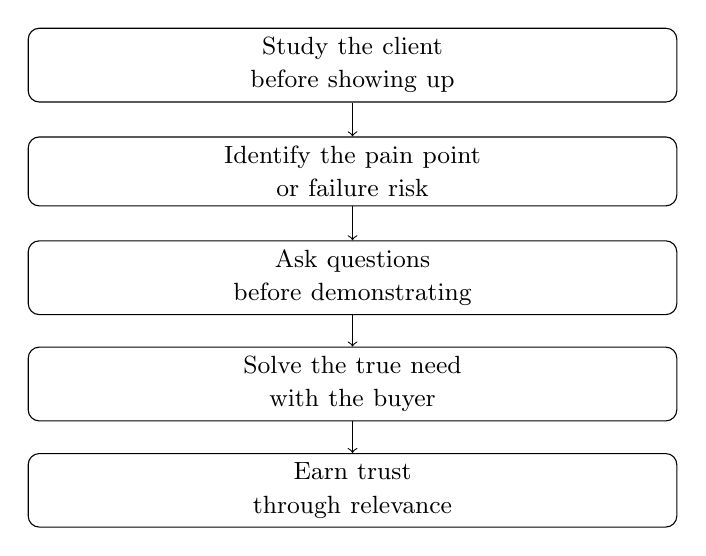
\begin{tikzpicture}[x=1cm,y=1cm]
\node[draw, rounded corners, text width=.66\linewidth, align=center] (a) at (0,0) {\small Study the client\\\small before showing up};
\node[draw, rounded corners, text width=.66\linewidth, align=center] (b) at (0,-1.35) {\small Identify the pain point\\\small or failure risk};
\node[draw, rounded corners, text width=.66\linewidth, align=center] (c) at (0,-2.7) {\small Ask questions\\\small before demonstrating};
\node[draw, rounded corners, text width=.66\linewidth, align=center] (d) at (0,-4.05) {\small Solve the true need\\\small with the buyer};
\node[draw, rounded corners, text width=.66\linewidth, align=center] (e) at (0,-5.4) {\small Earn trust\\\small through relevance};
\draw[->] (a) -- (b);
\draw[->] (b) -- (c);
\draw[->] (c) -- (d);
\draw[->] (d) -- (e);
\end{tikzpicture}
\end{figure}

This figure is a transcript-grounded reconstruction, not a board diagram. Its value is to preserve the order of operations. The temptation is to sell by adding more information. Williams's mechanism is to sell by removing irrelevance.

\section{The Folding-Paper Theory of Scale}

The next question asks how a business scales from six figures to seven, eight, and toward the scale of a large exit. Williams begins with valuation language:
\begin{equation}
EV \approx m_R R
\end{equation}
or
\begin{equation}
EV \approx m_E\,\mathrm{EBITDA}.
\end{equation}
Here \(EV\) denotes enterprise value, \(R\) denotes revenue, \(m_R\) denotes a revenue multiple, and \(m_E\) denotes an EBITDA multiple. This is a cautious standard notation for his phrase ``multiple of revenue or EBITDA.'' The transcript gives no actual multiple for HMS, so the notes should not invent one.

But the point of the answer is not valuation. Williams moves quickly from exit arithmetic to operating design. To scale, we first get the basics right: value proposition, total addressable market, customer, and key message. Then he asks for a moment to give a visual. The visual is a folding piece of paper: plan where the company is today, then plan what happens when it doubles, and then what happens when it doubles again.

\subsection{Question \& Answer}

\paragraph{Question.} How does a business scale without simply doing more of the same?

\paragraph{Answer.} It prepares the next operating design before the next scale state arrives. Let \(S_0\) denote the present scale of the business. Williams's doubling image can be represented as
\begin{equation}
S_0 \longrightarrow 2S_0 \longrightarrow 4S_0 \longrightarrow 8S_0.
\end{equation}
At every stage \(S_k\), there is an operating design \(D_k\):
\begin{equation}
D_k =
\{\mathrm{organization},\ \mathrm{metrics},\ \mathrm{alignment},\ \mathrm{relationships},\ \mathrm{channels}\}.
\end{equation}
The design is not decorative. It is the thing that prevents growth from becoming repeated improvisation.

\begin{figure}
\centering
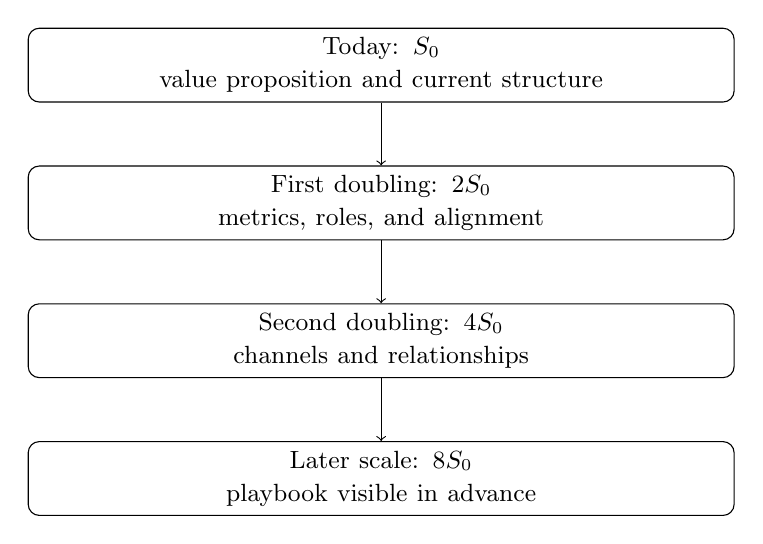
\begin{tikzpicture}[x=1cm,y=1cm]
\node[draw, rounded corners, text width=.72\linewidth, align=center] (s0) at (0,0) {\small Today: \(S_0\)\\\small value proposition and current structure};
\node[draw, rounded corners, text width=.72\linewidth, align=center] (s1) at (0,-1.75) {\small First doubling: \(2S_0\)\\\small metrics, roles, and alignment};
\node[draw, rounded corners, text width=.72\linewidth, align=center] (s2) at (0,-3.5) {\small Second doubling: \(4S_0\)\\\small channels and relationships};
\node[draw, rounded corners, text width=.72\linewidth, align=center] (s3) at (0,-5.25) {\small Later scale: \(8S_0\)\\\small playbook visible in advance};
\draw[->] (s0) -- (s1);
\draw[->] (s1) -- (s2);
\draw[->] (s2) -- (s3);
\end{tikzpicture}
\end{figure}

\paragraph{Worked example.} Suppose \(S_0\) denotes annual revenue and, for illustration only, \(S_0=\$1\,\mathrm{M}\). Then the folding-paper sequence gives
\begin{align}
S_0 &= \$1\,\mathrm{M},\\
2S_0 &= \$2\,\mathrm{M},\\
4S_0 &= \$4\,\mathrm{M},\\
8S_0 &= \$8\,\mathrm{M}.
\end{align}
The important mapping is not just from one revenue number to the next. It is from scale to design:
\begin{align}
S_0 &\mapsto D_0,\\
2S_0 &\mapsto D_1,\\
4S_0 &\mapsto D_2,\\
8S_0 &\mapsto D_3.
\end{align}
A weak scaling rule is
\begin{equation}
D_{k+1}=\text{whatever we invent after the pressure arrives}.
\end{equation}
Williams's stronger rule is
\begin{equation}
D_{k+1}=\text{the next design prepared while we are still operating at }D_k.
\end{equation}
That is the folding-paper theory. The future fold is already marked. When the company grows, the team is not forced to discover every structure for the first time.

\section{Career Capital and the Walk}

After scale, the conversation widens. The interviewer brings up Williams's book, \emph{Shift: A Playbook for Positive Change}. Williams says the working title was closer to \emph{Enjoy the Walk} or \emph{Enjoy the Journey}. This is a transition from enterprise mechanics to career mechanics.

Williams is sixty-three in the interview, still looking ahead, but he says the enduring value of a career is not simply the job title or company name. It is the skills learned and the people met. Mentors, colleagues, and people helped along the way become part of the compounding asset.

As a mnemonic, we can write career capital as
\begin{equation}
K_{\mathrm{career}}
=
K_{\mathrm{skills}}
+
K_{\mathrm{relationships}}
+
K_{\mathrm{reputation}}.
\end{equation}
This is not a transcript equation. It is a compact way to keep Williams's three-part claim from dissolving into a slogan. Skills matter. People matter. The reputation formed by helping people get better also matters.

\section{Work, Family, and Sharpening the Axe}

The next question asks whether work-life balance can coexist with success. Williams calls it a tough question, which is the right place to begin. The answer is not sentimental. It is operational.

He reports about
\begin{equation}
M_{\mathrm{American}} \approx 5.5\,\mathrm{M\ miles}
\end{equation}
on American Airlines. So the career involved heavy travel. His rule was simple: when away from family and home, work; when home, be home. He describes not taking calls all day Saturday and sometimes using Sunday night, after everyone had gone to bed, for about
\begin{equation}
T_{\mathrm{Sunday\ prep}} \approx 1\text{ to }1.5\ \mathrm{hours}
\end{equation}
of preparation.

\subsection{Question \& Answer}

\paragraph{Question.} Can work-life balance survive serious ambition?

\paragraph{Answer.} In this account, yes, but only as a discipline of attention. Balance is not the absence of hard work. It is knowing when work has the floor and when family has the floor. Williams's warning is that money by itself is thin. A person can retire with money but without family relationships, friendships, or a living network.

The mental-health question carries the same idea inward. Williams says a person needs more than one focus in life. His rhythm begins early:
\begin{equation}
t_{\mathrm{wake}} \approx 4{:}30,
\qquad
t_{\mathrm{gym}} \approx 5{:}00.
\end{equation}
He describes working out generally seven days a week, sometimes twice, and then names golf, sailing, hiking, and road biking as ways of getting away from the office.

The metaphor is sharpening the axe. If we have four hours to chop down a tree, the Lincoln saying tells us to spend the first three sharpening the axe. Williams uses the line as a performance model: renewal is not a reward after the work; it is part of the mechanism that makes the work sustainable.

\section{Risk, Trust, and Character Under Stress}

The interview then returns to biography. Williams studied computer science and began as a programmer. Early work in the field, programming devices and dealing with protocols, taught him not just technology but companies and people. That path leads through Arthur Andersen, healthcare technology, healthcare IBM consulting, and back to HMS Holdings and the \(\$3.5\) billion sale.

Only after that return to the origin story does the interviewer ask about the best and worst financial decision. Williams jokes that the worst was not buying enough Bitcoin or Tesla, but the more useful point comes next. He has lost money on an investment, but when he returned to the data available at the time and the people he was betting on, he still regarded the decision as reasonable.

So we should separate outcome from process:
\begin{equation}
\text{bad outcome} \not\Rightarrow \text{bad decision process}.
\end{equation}
That separation is central to commercial judgment. Venture risk is not eliminated by discipline; discipline decides which risks are worth taking.

Williams adds another rule:
\begin{equation}
\text{if every investment succeeds, the risk meter may be too low}.
\end{equation}
This is not a formal portfolio theorem. It is a qualitative claim about risk appetite. If a venture investor never fails, perhaps the portfolio never reached far enough into uncertainty.

\subsection{Question \& Answer}

\paragraph{Question.} What does due diligence miss if it stays inside the pitch deck?

\paragraph{Answer.} It misses character. Williams says to trust your gut and get to know people before investing with them. Not just through a demo. Not just through a PowerPoint presentation. Meet them, talk to them, get offline, and learn what they are made of. The reason is the sentence that anchors the whole section: no business plan goes off flawlessly.

We can write the diligence sequence as
\begin{equation}
\mathrm{Pitch}
\longrightarrow
\mathrm{Offline\ relationship}
\longrightarrow
\mathrm{Character}
\longrightarrow
\mathrm{Alignment}.
\end{equation}

\begin{figure}
\centering
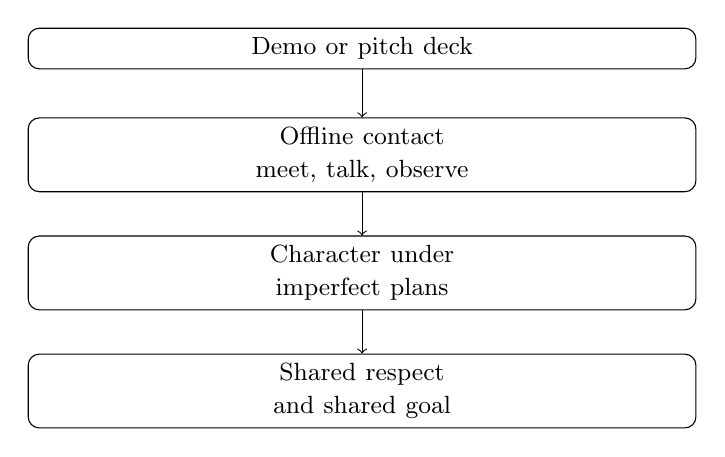
\begin{tikzpicture}[x=1cm,y=1cm]
\node[draw, rounded corners, text width=.68\linewidth, align=center] (a) at (0,0) {\small Demo or pitch deck};
\node[draw, rounded corners, text width=.68\linewidth, align=center] (b) at (0,-1.35) {\small Offline contact\\\small meet, talk, observe};
\node[draw, rounded corners, text width=.68\linewidth, align=center] (c) at (0,-2.85) {\small Character under\\\small imperfect plans};
\node[draw, rounded corners, text width=.68\linewidth, align=center] (d) at (0,-4.35) {\small Shared respect\\\small and shared goal};
\draw[->] (a) -- (b);
\draw[->] (b) -- (c);
\draw[->] (c) -- (d);
\end{tikzpicture}
\end{figure}

The transcript is badly corrupted during part of the later risk answer, so we should not reconstruct the missing example aggressively. The reliable endpoint is enough: different people have different risk profiles, and each person has to be comfortable with the profile they choose.

\section{Advice: Lift Others Up}

The closing question asks what Gen Z should know when starting careers and aspiring to leadership. Williams's answer is not to optimize first for advancement. Ask what you can do to help.

This closing advice is not disconnected from the earlier mechanics. It is the same trust mechanism moved into career form. Helping others creates trust; trust creates access; access creates chances to learn, sell, invest, and lead. A compact version is
\begin{equation}
\mathrm{Help}
\longrightarrow
\mathrm{Trust}
\longrightarrow
\mathrm{Opportunity}
\longrightarrow
K_{\mathrm{career}}.
\end{equation}
Williams warns that the more one is by oneself, the more one will be by oneself. That is not just moral advice. It is a network claim. Careers compound through other people.

\section{Summary}

Williams's interview unfolds as a sequence of operating judgments. First we locate the investment stage: a \(\$50\) million venture pool, early checks, and companies still below roughly \(\$2\) million in revenue. Then we see why focus matters: smart founders still need a message that lands. Sales becomes diagnosis, not demonstration. Scale becomes a predesigned sequence of doublings, not just more effort. Career capital becomes skills plus relationships plus reputation. Work-life balance becomes disciplined attention. Risk becomes the study of people under imperfect plans. The final advice gathers the pieces into one rule: help others, because trust is the medium through which opportunity travels.